\chapter{Theoretische Grundlagen}
\label{chap:theorie}

%%%% Ein kleines Chapter zur schwachen WW??

\section{Geschichte der Neutrinos}
\label{sec:neutrinogeschichte}

Neutrinos wurden erstmals am $4.$ Dezember $1930$ von Pauli als Spin-$\frac{1}{2}$-Teilchen postuliert, um das Problem der Drehimpulserhaltung und das kontinuierliche Elektronenspektrum beim $\beta$-Zerfall zu lösen. %\cite{zuber}
Er führte das Neutrino als Teilchen ein, dass beim $\beta^-$-Zerfall
\begin{equation*}
    n \rightarrow p + e^- + \bar{\nu}_e
\end{equation*}
gemeinsam mit dem Elektron emittiert wird, anders als dieses allerdings nicht detektierbar ist. \\
Diese Annahme Paulis wurde lange kritisch betrachtet, bis Neutrinos in den $50$er Jahren in Atomreaktoren zweifellos nachgewiesen werden konnten. %\cite{zuber}\\

Im Standardmodell der Teilchen sind Neutrinos als einzige masselose, elektrisch neutrale Leptonen vertreten.
Theoretisch lassen sie sich durch die Wellenfunktionen $\psi$ als lorentzinvariante Lösung der relativistischen Diracgleichung
\begin{equation}
    \left(i \gamma_\mu \frac{\partial}{\partial x_\mu} - m \right) \psi = 0
    \label{eq:dirac}
\end{equation}
beschreiben.
Die Wellenfunktion ist dabei ein vierkomponentiger Spinor, $\gamma_\mu$ sind die $4 \times 4$-Gammamatrizen in Diracdarstellung mit
\begin{align}
    \gamma^0_\text{Dirac} = \left( \begin{array}{c c}
        \mathbb{1} & 0          \\ 
        0          & -\mathbb{1} \\ 
        \end{array}\right) \,,
    &&
    \gamma^k_\text{Dirac} = \left( \begin{array}{c c}
        0           & \sigma_k  \\ 
        -\sigma_k   & 0         \\ 
        \end{array}\right) \,,
    \label{eq:gammamatrizen}
\end{align}
wobei $\mathbb{1}$ die Einheitsmatrix und $\sigma_k$ mit $k = 1, 2, 3$ die $2 \times 2$-Paulimatrizen
\begin{align}
    \sigma_1 = \left( \begin{array}{c c}
        0 & 1   \\ 
        1 & 0   \\ 
        \end{array}\right) \,,
    &&
    \sigma_2 = \left( \begin{array}{c c}
        0           & -i  \\ 
        i  & 0         \\ 
        \end{array}\right) \,,
    &&
    \sigma_3 = \left( \begin{array}{c c}
        1           & 0 \\ 
        0   & -1         \\ 
        \end{array}\right)
    \label{eq:paulimatrizen}
\end{align}
darstellen. 

Somit sind Neutrinos auch die einzigen Leptonen, die nicht nur nicht stark wechselwirken, sondern auch nicht an der elektromagnetischen Wechselwirkung teilnehmen.
Tatsächlich ist ihre Wechselwirkung mit Materie so gering, dass die $7 \cdot 10^{10}$  Neutrinos, die pro $\si{\centi\meter}^2$ und pro Sekunde auf die Erde treffen, keinerlei Auswirkung
auf das Leben ihrer Bewohner haben \cite[S. ~133]{grupen}. 

Zu jeder der drei Leptonengenerationen, sprich Elektronen, Myonen und Tauonen existiert dabei ein korrespondierendes Neutrino.
Dieser sogenannte Flavour eines Neutrinos ist dabei nicht fest, sondern kann sich zeitlich und räumlich periodisch ändern.
Die Entdeckung dieser sogenannten Neutrinooszillationen erhielt im Jahre $2015$ den Nobelpreis \cite[S. ~19]{oberauer}.



\section{Neutrinos und spontane Symmetriebrechung}

Um die Masse der Neutrinos zu erklären, führen wir ein Quantenfeld ein, das Majoronenfeld, welches die Leptonenzahlsymmetrie, wenn auch nur geringfügig, bricht.
Dazu sollen hier zunächst einige Begrifflichkeiten geklärt werden.

\subsection{Das Eichprinzip} %\cite{kleingrot}

Das Prinzip der Eichinvarianz beschreibt Transformationen, die die Physik eines Systems, also die Lagrangedichte, invariant lassen.
Dabei unterscheiden wir zwischen globalen Transformationen, die sich, unabhängig von Raum und Zeit, überall gleichartig auf das System auswirken und lokalen Eichtransformationen, 
die von Ort und Zeit abhängig unterschiedlich auf das System wirken.

Für uns sind im Folgenden insbesondere die globalen Symmetrien relevant.
Jede dieser globalen Symmetrien, ist durch das Noether-Theorem mit einer Erhaltungsgröße verknüpft.
Unter globale Transformationen fallen beispielsweise die Multiplikation der Lösung $\psi$ der Schrödingergleichung um eine konstante komplexe Phase $\mathrm{e}^{i \alpha}$.

\subsection{Spontane Symmetriebrechung} %\cite{kleingrot}


Der Mechanismus der spontanen Symmetriebrechung erlaubt uns, massebehaftete Eichbosonen einzuführen, ohne die Eichinvarianz der Lagrangedichte durch explizite Massenterme zu verlieren.
Konkret sprechen wir von einer spontanen Symmetriebrechung, wenn die grundlegenden Gleichungen eines Systems über eine Symmetrie verfügen, der der Grundzustand nicht folgt.

Das Majoronenfeld, also auch die dazugehörigen Eichbosonen, die Majoronen, lässt sich durch ein Potential einführen, dessen Vakuumerwartungswert (VEV), also der Zustand niedrigster Energie $E_\text{min}$ verschieden von null ist. \\
Wir fordern also, dass unser System, beschrieben durch den Hamiltonian $H$, invariant unter einer Transformation $U$ bleibt, sprich der Kommutator $[H, U]$ verschwindet.
Es gilt also auch
\begin{equation*}
    H U \ket{0} = U H \ket{0} = E_\text{min} U  \ket{0} 
\end{equation*}
und damit
\begin{equation*}
    U \ket{0}_i = \ket{0}_j \,, \quad i \neq j \,,
\end{equation*}
sofern mehrere entartete Zustände $\ket{0}_i$ existieren. \\
Die Transformation $U$ lässt das Vakuum $\ket{0}$ also nicht notwendigerweise invariant.

Das einfachste Potential mit diesen Eigenschaften besitzt die Form
\begin{equation}
    V(x) = -\frac{1}{2} \mu^2 x^2 + \frac{1}{4} \lambda x^4 \,, \quad \mu,\lambda > 0 \,.
\end{equation}
Offensichtlich ist dieses, auch Mexico-Hut-Potential genannte, Potential radialsymmetrisch.
Es existiert also ein Kreis mit Radius
\begin{equation*}
    x_0 = \sqrt{\frac{\mu^2}{\lambda}} \,,
\end{equation*}
auf dem die Zustände minimaler Energie verteilt sind.
\autoref{fig:mexicohutpot} zeigt eine Darstellung des Potentials in zwei Dimensionen.

\begin{figure}[H]
    \centering
    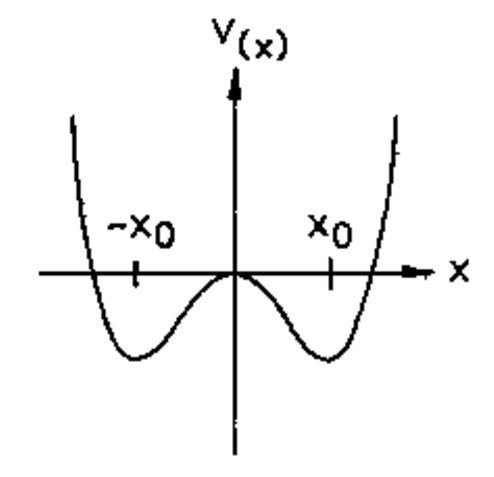
\includegraphics[]{figures/MexicoHutpotential.pdf}
    \caption{Darstellung des Mexico-Hut-Potentials in zwei Dimensionen. Zu erkennen sind die zwei möglichen Grundzustände $x = \pm x_0$ \cite{kleingrot}.}
    \label{fig:mexicohutpot}
\end{figure}

Anschaulich stellen wir uns vor, dass wir uns zunächst im Zentrum des Potentials befinden.
Von diesem Punkt aus besitzt das Potential eine globale Symmetrie, egal in welche Richtung wir schauen.
Betrachten wir das ganze aber von einem der Vakua, existiert diese Symmetrie unter der Transformation $x \rightarrow -x$ nicht länger.

\section{Ursprung der Neutrinomasse} %\cite{kleingrot}
\label{sec:neutrinomasse}

Als nur schwach wechselwirkende Teilchen ist zum jetzigen Zeitpunkt nur die Existenz linkshändiger Neutrinos $\nu_L$ und rechtshändiger Antineutrinos $\bar{\nu}_R$ bewiesen.
Diese sind über die Ladungs- und Paritätskonjugation $C P$ durch 
\begin{equation}
    (\nu_L)^{C P} = \bar{\nu}_R
    \label{eq:cpkonju}
\end{equation}
miteinander verknüpft.
Der Paritätsoperator $P$ transformiert dabei linkshändige in rechtshändige Teilchen und umgekehrt, die Ladungskonjugation überführt Teilchen in ihre Antiteilchen, ohne dabei ihre Händigkeit zu verändern.
Sind die ladungskonjugierten Teilchen zu $\nu_L$ bzw. $\bar{\nu}_R$ bisher nicht beobachtete, unabhängige Teilchen, sprechen wir von einem Dirac-Neutrino.
Ist $\nu_L$ bzw- $\bar{\nu}_R$ sein eigenes ladungskonjugiertes Teilchen, gilt also
\begin{align*}
    (\nu_L)^C = \nu_L \,, && (\bar{\nu}_R)^C = \bar{\nu}_R \,.
\end{align*}
Diese, nach dem italienischen Physiker Ettore Majorana benannten Majorana-Neutrinos lösen nach wie vor die Diracgleichung \eqref{eq:dirac}, es existieren allerdings nur zwei physikalisch unterscheidbare Zustände.
Diese beiden Majorana-Masseneigenzustände
\begin{align*}
    \nu_1 = \nu_L + \nu^{C P}_R \\
    \nu_2 = \nu_R + \nu^{C P}_L
\end{align*}
sind ihre eigenen Antiteilchen und bilden gemeinsam den Massenterm der Lagrangedichte $\mathcal{L}_M$ zu
\begin{equation}
    \mathcal{L}_M = \mathcal{L}^L_M + \mathcal{L}^R_M = -\frac{1}{2} m^M_L \bar{\nu}_1 \nu_1 - \frac{1}{2} m^M_R \bar{\nu}_2 \nu_2 \,.
    \label{eq:lagrangedichtemajo}
\end{equation}
Dabei stellen $m^M_L$ bzw. $m^M_R$ als Massen die Kopplungsstärken zwischen $\nu_L$ und $\bar{\nu}_R$ bzw. $\nu_R$ und $\bar{\nu}_L$ dar.

Im Standardmodell ordnet der Leptonenzahloperator $L$ jedem Lepton die Leptonenzahl $+1$ und jedem Antilepton die Leptonenzahl $-1$.
So erhalten auch Neutrinos im Standardmodell eine Leptonenzahl. 
Sind jetzt jedoch, wie oben beschrieben, Neutrinos und Antineutrino als Majoranateilchen identisch, ergibt die Zuordnung einer Leptonenzahl keinen Sinn mehr.
Die globale Leptonenzahlsymmetrie ist also, wenn auch nur sehr geringfügig, spontan gebrochen.

\section{Neutrinos und Neutrinomischung in verschiedenen Basen}
\label{sec:neutrinobasen}

\subsection{Flavourbasis} %\cite[Kap. 2.1]{oberauer}
\label{subsec:flavourbasis}
Voraussetzung für die Neutrinooszillationen ist aber, dass Masseneigenzustände $\nu_i$ als Lösungen der Diracgleichung mit den Masseneigenwerten $m_i \neq 0 (i = 1, 2, 3)$ existieren.
Diese Masseneigenzustände bestimmen die Propagation des Neutrinos im Vakuum und müssen nicht zwangsläufig identisch zu den Flavoureigenzuständen sein.
Hier betrachten wir die Flavoureigenzustände $\nu_\alpha (\alpha = e, \mu, \tau)$ als Superposition der Masseneigenzustände mit
\begin{equation}
    \nu_\alpha = \sum_i U_{\alpha i} \nu^{(h_i)}_i \,,
    \label{eq:flavourbasis}
\end{equation}
wobei $U_{\alpha i}$ die unitäre Mischungsmatrix zwischen Massenbasis und Flavourbasis darstellt \cite[Kap. 2.1]{oberauer}.
Das Superskript $(h_i) = \pm 1$ beschreibt dabei die Helizität des Eigenzustands.

\subsection{Materiebasis} %\cite{päspaper}
\label{subsec:materiebasis}

Das Material im Inneren eines Stern wird im Laufe seines Lebens zu immer schwereren Elementen fusioniert und setzt große Mengen an Energie frei.
Normalerweise reicht der so entstehende Strahlungsdruck, um dem äußeren Gravitationsdruck standzuhalten.
Erreicht der Stern jedoch mit Eisen das Ende der Fusionskette, sinkt der Strahlungsdruck immer weiter, bis der Kern das Chandrasekhar-Limit erreicht und der Stern endgültig instabil wird.
Besitzt der Stern eine ausreichende Gesamtmasse, implodiert er bis zu einer kritischen Dichte.
Sobald diese Dichte im Stern herrscht, entsteht eine Schockwelle im Inneren, die das Sternmaterial nach außen katapultiert.

Dabei wird ein großer Teil der Supernovaenergie durch Neutrinos propagiert.
Ist es diesen nun möglich, bei der Propagation durch das Supernovamedium über den Zerfall $\tilde{\nu}^{(h_i)}_i (p_i) \rightarrow \tilde{\nu}^{(h_j)}_j (p_j) + J(q)$
Energie in Form von Majoronen $J$ mit Impuls $q$ abzustrahlen, kann sich, je nach Kopplungsstärke zwischen Neutrino und Majoron, das Energiespektrum der Supernova verändern.
Diese Stöße wirken sich auf das Oszillations- und Propagationsverhalten der Neutrinos aus und können mithilfe der Materiebasis beschrieben werden.

Drücken wir dabei das linkshändige vierkomponentige Feld $\nu_L$ in chiraler Darstellung der Gammamatrizen über ein zweikomponentiges Feld $\phi$ mit $\nu^T_L = (\phi, 0)^T$ aus, 
näheres dazu findet sich in \cite{komponentendinger}, lässt sich der Lagrangian in der Materiebasis als
\begin{equation}
    \mathcal{L}_\text{tot} = \mathcal{L}_0 + \mathcal{L}_\text{med} + \mathcal{L}_\text{int}
    \label{eq:materielagrange}
\end{equation}
mit
\begin{align*}
    \mathcal{L}_0          &=   i \sum_i \left[\phi^\dagger_i \left(\partial_t - \vec{\sigma} \times \nabla \right) \phi_i - \frac{m_i}{2} \left(\phi^T_i \sigma_2 \phi - \phi^\dagger_i \sigma_2 \phi^*_i\right) \right] \,,\\
    \mathcal{L}_\text{med} &= - \sum_{i j} \phi^\dagger_i V_{i j} \phi_j  \,,\\
    \mathcal{L}_\text{int} &= - J \sum_{i j} g^M_{i j} \left( \phi^T_i \sigma_2 \phi_j + \phi^\dagger_i \sigma_2 \phi^*_j \right)
\end{align*}
schreiben \cite{päspaper}.
Dabei beschreibt der freie Lagrangian $\mathcal{L}_0$ die Propagation im Vakuum, $\mathcal{L}_\text{med}$ die in der Potentialmatrix $V$ berücksichtigten Effekte von Materie und $\mathcal{L}_\text{int}$
beschreibt Wechselwirkungen zwischen Neutrinos und Majoronen.
Die Kopplungsstärke zwischen Majoronen und Neutrinos der Massenbasis ist dabei in $g^M_{i j}$ zusammengefasst, $\vec{\sigma} = (\sigma_1, \sigma_2, \sigma_3)$ denotiert den Vektor der in \eqref{eq:paulimatrizen} zu findenden Paulimatrizen
und $m_i$ den Masseneigenwert des jeweiligen Neutrinos in der Massenbasis.

Für gewöhnlich würden wir hier, um die Eigenzustände des bereits erwähnten Zerfalls $\tilde{\nu}^{(h_i)}_i (p_i) \rightarrow \tilde{\nu}^{(h_j)}_j (p_j) + J(q)$ zu bestimmen, 
die aus $\mathcal{L}_\text{tot}$ resultierenden Feldgleichungen 
\begin{equation}
    i \left(\partial_t - \vec{\sigma} \times \nabla \right) \phi_i + i m_i \sigma_2 \phi^*_i - \sum^3_j V_{i j} \phi_j = 0 \,,
\end{equation}
wie in \cite{komponentendinger} gezeigt, mithilfe von Planarwellenspinoren definiter Helizität lösen, 
allerdings stimmen die so erhaltenden Lösungen mit den aus der Diagonalisierung der Mikheyev-Smirnov-Wolfenstein-Gleichung folgenden Lösungen überein.
Sie beschreibt die Zeitentwicklung schwacher Eigenzustände und die Mischung zwischen diesen und den Energieeeigenzuständen durch
\begin{equation}
    i \partial_t \nu^{(h)}_i = \left(H^\text{rel}_{i j} + U_{i \alpha} V_{\alpha \beta} U^\dagger_{\beta j}\right) \nu^{(h)}_j \,.
    \label{eq:MSW-gleichung}
\end{equation}
Aufgrund der geringen Massen und hohen Energien der Neutrinos, bei denen auch Energie- und Materieeigenzustände übereinstimmen, betrachten wir den hochrelativistischen Limes des Hamiltonians $H^\text{rel}_{i j} \approx \left(p + \frac{m^2_i}{2 p}\right) \delta_{ij}$ mit dem Kronecker-$\delta$
\begin{equation}
    \delta_{ij} = \begin{cases}
                    1, \quad i=j \\
                    0, \quad \text{sonst} \,.
                  \end{cases}
                  \label{eq:kronecker}
\end{equation}
$V$ ist dabei die diagonale Potentialmatrix der schwachen Basis, also
\begin{equation}
    V = \left( \begin{array}{c c c}
        V_C + V_N   &   0     &     0   \\ 
        0           &   V_N   &     0   \\ 
        0           &   0     &     V_N  \\
        \end{array}\right) \,,
\end{equation}
wobei $V_C = \sqrt{2} h G_F n_B (Y_\text{e}) + Y_{\nu_\text{e}}$ das von geladenen Strömen, also schwachen Wechselwirkungen, bei denen ein $W^+$- oder $W-$- Boson ausgetauscht wird erzeugte und 
$V_N = \sqrt{2} h G_F n_B \left(-\frac{1}{2} Y_N + Y_{\nu_\text{e}}\right)$ das durch ungeladene Ströme, also nur unter Austausch von neutralen $Z$-Bosonen stattfindende schwache Wechselwirkungen erzeugte Potential.
Mit der Baryonendichte $n_B$ des betrachteten Mediums gilt für ein beliebiges Teilchen $i$ mit korrespondierendem Antiteilchen $\bar{i}$ $Y_i = \frac{n_i - n_{\bar{i}}}{n_B}$.

Aus der Diagonalisierung der rechten Seite der MSW-Gleichung folgen die Materieeigenzustände
\begin{equation}
    \tilde{\nu}^{(h_i)}_i = \sum_i \tilde{U}_{i j} \nu^{(h_j)}_j \,.
    \label{eq:materiebasis}
\end{equation} 
Ähnlich wie die Flavoureigenzustände lassen sie sich als Superposition der Masseneigenzustände beschreiben.
Sie unterscheiden sich lediglich in der Mischungsmatrix $\tilde{U}$.

Hier können wir die in \autoref{subsec:flavourbasis} auftretende Mischungsmatrix $U$ als
\begin{equation}
    U = U_{2 3} \, U_{1 3} \, U_{1 2} \, U_0
    \label{eq:kopplungflavour}
\end{equation}
parametrisieren.
Bei den Matrizen $U_{i j}$ handelt es sich dabei um Rotationsmatrizen, die in der $i j$-Ebene eine Rotation um den Winkel $\theta_{i j}$ durchführen.
Die in \autoref{sec:neutrinomasse} behandelte mögliche CP-Verletzung findet sich als Phase in der Matrix $U_0$ wieder.

Wie in \cite{theta13} festgestellt ist $\theta_{1 3}$ nicht, wie lange Zeit angenommen, null.
Nach aktuellen Daten der Particle Data Group gilt $\sin^2 \left(\theta_{1 3} \right) = \num{2.20 +- 0.07} \cdot 10^{-2}$ \cite{neutrinospdg}, hier wird $\theta_{1 3}$ dennoch auf null gesetzt.

Damit vereinfacht sich die Mischungsmatrix zu $U = U_{2 3} \, U_{1 2} \, U_0$.
Jetzt können wir $\theta_{1 2}$ als solaren Mischungswinkel $\theta_\odot$ und $\theta_{2 3}$ als atmosphärischen Mischungswinkel $\theta_\text{atm}$ identifizieren.
Da zusätzlich, vor allem für leichte Neutrinos in der Nähe der Neutrinosphäre der Supernova, $|V_{\alpha \alpha}| \gg \frac{m^2_i}{2 p}$ für alle Elemente der Potentialmatrix gilt, unterscheiden sich die Materieeigenzustände nur um eine
beliebige Drehung $\theta'$ in der $\nu_\mu$ - $\nu_\tau$ Ebene von den Eigenzuständen der schwachen Basis.
Wir wählen $\theta' = -\theta_\text{2 3}$, um möglichst einfache Ausdrücke der Materieeigenzustände zu erhalten, wie sie in \autoref{tab:materieeigis} dargestellt sind.
\begin{table}[H]
    \centering
    \begin{tabular}{S S S}
      \toprule
    {Materieeigenzustände $\tilde{\nu}^{(h_i)_i}$} & {Schwache Eigenzustände $\nu_{\alpha'}$} & {Potential $V$} \\
      \midrule
       {$\tilde{\nu}^+_1$} & {$\bar{\nu}_e$}                                                        &  {$- (V_C + V_N)$} \\
       {$\tilde{\nu}^+_2$} & {$\bar{\nu}_{\mu'}  = c_{2 3} \bar{\nu}_\mu - s_{2 3} \bar{\nu}_\tau$} &  {$- V_N$} \\
       {$\tilde{\nu}^+_3$} & {$\bar{\nu}_{\tau'} = s_{2 3} \bar{\nu}_\mu + c_{2 3} \bar{\nu}_\tau$} &  {$- V_N$} \\
       {$\tilde{\nu}^-_1$} & {$\nu_{\mu'}        = c_{2 3} \nu_\mu       - s_{2 3} \nu_\tau$}       &  {$V_N$} \\
       {$\tilde{\nu}^-_2$} & {$\nu_{\tau'}       = s_{2 3} \nu_\mu       + c_{2 3} \nu_\tau$}       &  {$V_N$} \\
       {$\tilde{\nu}^-_3$} & {$\nu_e$}                                                              &  {$V_C + V_N$} \\
    \bottomrule
    \end{tabular}
    \caption{Materieeigenzustände $\tilde{\nu}^\pm_i$ positiver und negativer Helizität im Limes $|V_{\alpha \alpha}| \gg \frac{m^2_i}{2 p}$ als Rotation der schwachen Eigenzustände. Die Eigenzustände sind dabei so
            angeordnet, dass das Potential in der Tabelle nach unten hin ansteigt. Es gilt $c_{2 3} = \cos(\theta_{2 3})$ und $s_{2 3} = \sin(\theta_{2 3})$.}
    \label{tab:materieeigis}
\end{table}

Genauso lassen sich auch die Kopplungsmatrixelemente $\tilde{g}_{i j}$ der Materiebasis als Rotation der Elemente der schwachen Basis identifizieren.
In den hier betrachteten Modellen ist die schwache Kopplungsmatrix diagonal, es gilt also
\begin{equation}
    g^W = \left( \begin{array}{c c c}
        g_1         &   0     &     0   \\ 
        0           &   g_2   &     0   \\ 
        0           &   0     &     g_3  \\
    \end{array}\right) \,.
    \label{eq:schwachekopplung}
\end{equation}

Damit ist also
\begin{equation}
    g_{\alpha' \beta'} \equiv \ \tilde{g}_{i j} = U(-\theta_{2 3}) \, g^W_{\alpha \beta} \, U^T(-\theta_{2 3}) = U_{1 2} \, U^*_0 \, g^M_{i j} \, U^\dagger_0 \, U_{1 2} \,,
\end{equation}
wenn wir zusätzlich benutzen, dass die schwache Kopplungsmatrix und die der Massenbasis über $g^W = U \, g^M \, U^T$ verknüpft sind, oder explizit
\begin{align}
    \tilde{g} &= \left( \begin{array}{c c c}
        g_{ee}                  &   g_{e \mu'}          &     g_{e \tau'}       \\ 
        g_{e \mu'}              &   g_{\mu' \mu'}       &     g_{\tau' \mu'}    \\ 
        g_{e \tau'}             &   g_{\tau' \mu'}      &     g_{\tau \tau}     \\
    \end{array}\right) \nonumber\\
    &= \left( \begin{array}{c c c}
        g_1 \cos^2 \theta_\odot + g_2 sin^2 \theta_\odot \mathrm{e}^{-2 i \delta}                   &   \frac{1}{2} \left(-g_1 + g_2 \mathrm{e}^{-2 i \delta}\right) \sin(2 \theta_\odot)       &     0   \\ 
        \frac{1}{2} \left(-g_1 + g_2 \mathrm{e}^{-2 i \delta}\right) \sin(2 \theta_\odot)           &   g_1 sin^2 \theta_\odot + g_2 \cos^2 \theta_\odot\mathrm{e}^{-2 i \delta}                &     0   \\ 
        0                                                                                           &   0                                                                                       &     g_3  \\
    \end{array}\right)
    \label{eq:materiekoppmat}
\end{align}
mit der CP-verletzenden Phase $\delta$.
Die Kopplungsparameter $g_2$ und $g_3$ lassen sich dabei in Abhängigkeit von $g_1$ und $m_1$, also der Masse des ersten Masseneigenzustands, ausdrücken als
\begin{align}
    g_2 = g_1 \sqrt{1 + \frac{\Delta m^2_\odot}{m^2_1}}\,, && g_3 = g_1 \sqrt{1 + \frac{\Delta m^2_\odot + \Delta m^2_\text{atm}}{m^2_1}} \,,
    \label{eq:g2g3}
\end{align}
wobei wir die Definitionen $\Delta m^2_{1 2} = \Delta m^2_\odot$ und $\Delta m^2_{23} = \Delta m^2_\text{atm}$ benutzen.
So ist also ein Zusammenhang der Kopplungsmatrizen aller drei Basen hergestellt, der im folgenden genutzt werden kann, um die Einschränkungen auf die Kopplungsstärken deutlich zu machen.
















